\documentclass{article}
\usepackage[landscape]{geometry}
\usepackage[utf8]{inputenc}
\usepackage{tikz}
\usetikzlibrary{mindmap,backgrounds}
\pagestyle{empty}
\usepackage[T1]{fontenc}
\usepackage[utf8]{inputenc}
%lmodern	lmss
\usepackage{helvet}

\begin{document}
\pagestyle{empty}


{\fontfamily{hvt}
\centering
\begin{figure}
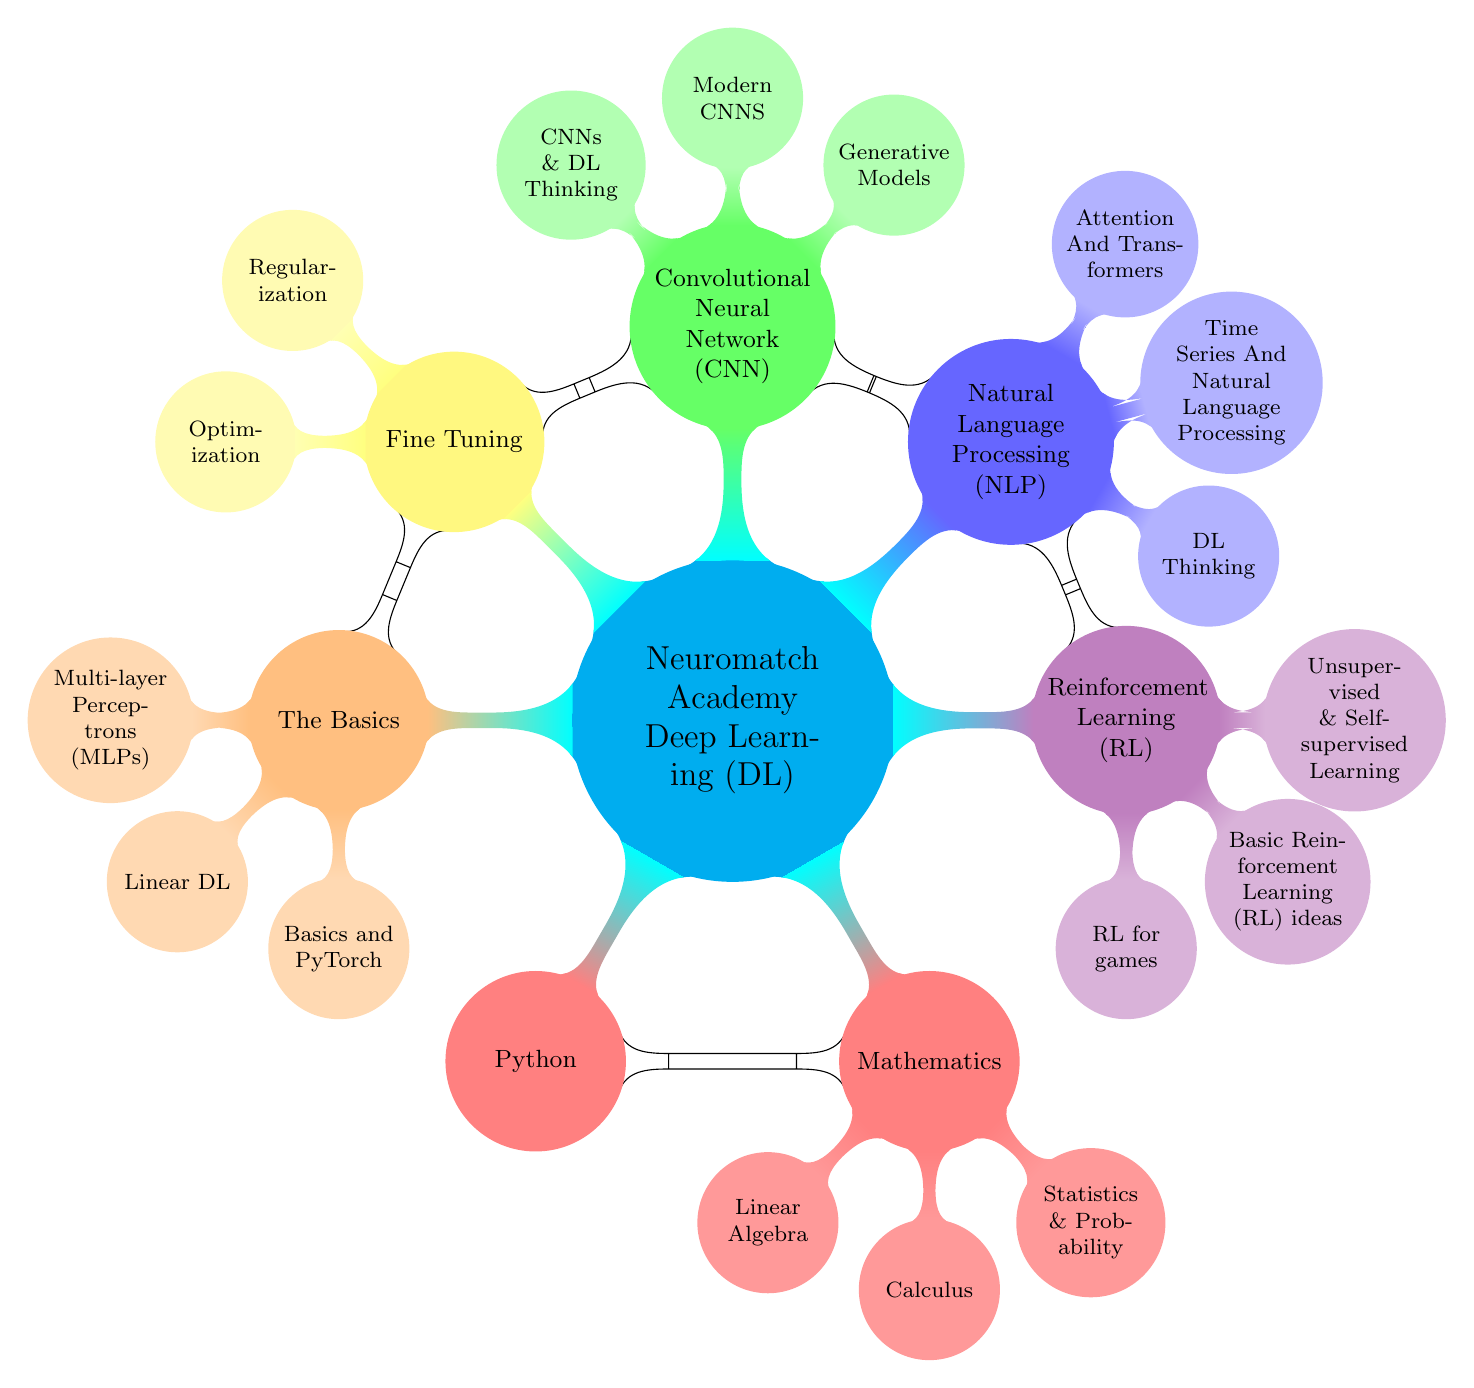
\begin{tikzpicture}




  
  \path[mindmap,concept color=cyan,text=black]
    node[concept,concept color=cyan!100](pde) {Neuromatch Academy \\ Deep Learning (DL)} 
    child[grow=240,concept color=red!50] { node[concept](Pyth) {Python} 
    }   
    child[grow=300,concept color=red!50]{node[concept] (Math){ Mathematics}    
    child[grow=225, concept color=red!40] {
      node[concept](LinAl) {Linear Algebra}
    }
    child[grow=270,concept color=red!40] { node[concept](Cal) {Calculus} }
    child[grow=315,concept color=red!40] { node[concept](Stats) {Statistics \& Probability} 
    }
    }
        % THE BASICS
             child[grow=180,concept color=orange!50]{node[concept] (TheBasics){The Basics}
      % ModTy
      child[grow=270,concept color=orange!30]{node[concept] (IntroDL){Basics and PyTorch}    }
      child[grow=225,concept color=orange!30]{node[concept] (DLLinear){Linear DL}}
      child[grow=180,concept color=orange!30]{node[concept] (MLP){Multi-layer Perceptrons (MLPs) }}
    }
            % Fine Tuning
             child[grow=135,concept color=yellow!50]{node[concept] (FineTuning){Fine Tuning}
      % ModTy
      child[grow=180,concept color=yellow!30]{node[concept] (Opt){Optim-\\ization}    }
      child[grow=135,concept color=yellow!30]{node[concept] (Reg){Regular-\\ization
}}
    }
    % CNN
       child[grow=90,concept color=green!60]{node[concept] (CNN){Convolutional Neural Network (CNN)}
   child [grow=135,concept color=green!30]
    {node [concept] (ParamShar) {CNNs \& DL Thinking}
    }
    child [grow=90,concept color=green!30]
    {node [concept] (ModConv) {Modern CNNS}
    }
     child [grow=45,concept color=green!30]
    {node [concept] (ModRNN) {Generative Models}
    }
   }
       % NLP
       child[grow=45,concept color=blue!60]{node[concept] (NLP){Natural Language Processing (NLP)}
   child [grow=60,concept color=blue!30]
    {node [concept] (ParamShar) {Attention And Transformers}
    }
    child [grow=15,concept color=blue!30]
    {node [concept] (ModConv) {Time Series And Natural Language Processing}
    }
     child [grow=-30,concept color=blue!30]
    {node [concept] (ModRNN) { DL Thinking}
    }
   }
     % Reinforcement Learning (RL)
     child[grow=0,concept color=violet!50]{node[concept] (RL){ Reinforcement Learning (RL) }
   child[grow=0,concept color=violet!30]{node[concept] (Unsup){Unsuper- \\ vised \& Self-supervised Learning }    }
 child[grow=-45,concept color=violet!30]{node[concept] (BasRL){Basic Reinforcement Learning (RL) ideas}
   }
   child[grow=-90,concept color=violet!30]{node[concept] (RLgames){RL for games}
   }
    };

   \begin{pgfonlayer}{background}
    \draw [circle connection bar]
      (FineTuning) edge (CNN)
      (CNN) edge (NLP)
      (NLP) edge (RL)
      (TheBasics) edge (FineTuning) 
      (Pyth) edge (Math)
      ;
  \end{pgfonlayer}
\end{tikzpicture}

\end{figure}
}
\end{document}

